\documentclass{article}
%\usepackage{geometry}
% \geometry{top = 1in, bottom = 1in, left = 1in, right = 1in}
\usepackage[top = 0.7in, bottom = 0.7in, left = 0.7in, right = 0.7in]{geometry}
\usepackage{amsmath,amssymb,amsthm,mathrsfs}
\usepackage{graphicx}
\usepackage{bm}
\usepackage{float}
\usepackage[font=footnotesize,labelfont=bf]{caption}

\usepackage{fancyhdr}
\pagestyle{fancy}
\rhead{\footnotesize {07/28/2012 ; MESA version 4028} }
\chead{\footnotesize {Authors: Jared Brooks, Lars Bildsten, Bill Paxton} }
\lhead{\footnotesize {mesa/star/test\_suite/wd\_ignite} }

\begin{document}
	
	\begin{center}
		\begin{Large}
		       \textbf{WD IGNITE}\\
		\end{Large}
	\end{center}
	

        This test is to show a white dwarf undergoing ignition of core carbon and oxygen as it nears the Chandrasekhar mass limit.  Therefore, the test should be cut off when the total power from all nuclear reactions is $10^8$ $L_\odot$ (\texttt{power\_nuc\_burn\_u\-pper\_limit = 1d8}).\\

	Here we start with a 1 $M_\odot$ carbon-oxygen white dwarf, which slowly accretes material over 400 Myr (a rate of $1\times10^{-9}$ $M_\odot$/yr), composition of accreted material listed below.\\

	\noindent Accreted Material composition (mass fractions):
        \begin{itemize}
        \item $^{12}$C: 0.25
        \item $^{16}$O: 0.75
        \end{itemize}

        The plot to the left (figure \ref{fig:1}) shows a constant rate of mass accretion, taking it from 1 $M_\odot$ to near the Chandrasekhar mass limit.  The profile to the right (figure \ref{fig:2}) shows the initial abundance of each element present by mass fraction.  This shows that the white dwarf is almost entirely carbon and oxygen.  (Note: The Ne20 shown here actually represents Ne22, this is because \texttt{MESA} is using a simplified nuclear reaction network.)

	\begin{figure}[H]
          \begin{minipage}[b]{0.5\linewidth}
	    \centering
	    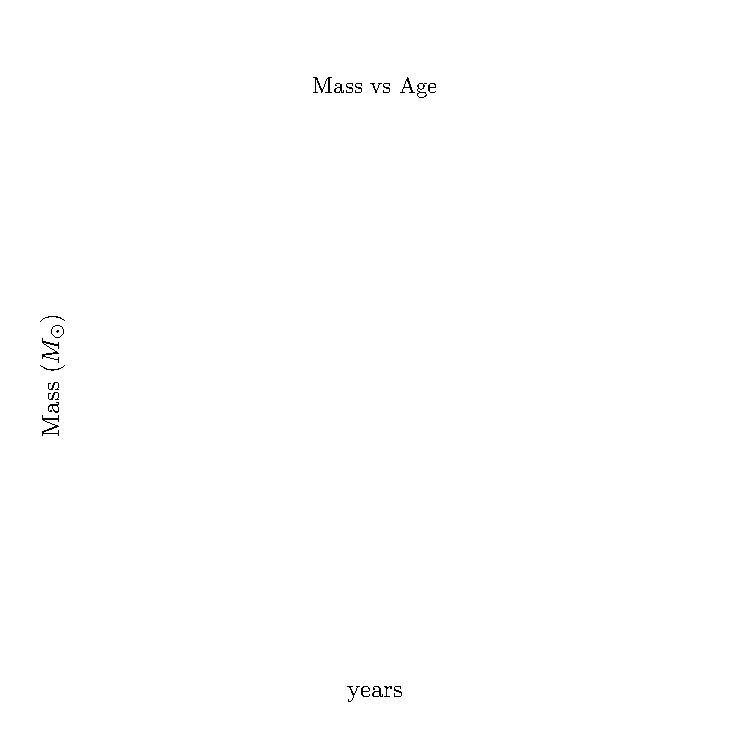
\includegraphics[width = 3.8in]{/Users/jaredbrooks/wd_ignite/plots_out/Mass_vs_Age.pdf}
	    \caption{Constant mass accretion rate until near Chandrasekhar mass limit}
	    \label{fig:1}
          \end{minipage}
          \hspace{0cm}
          \begin{minipage}[b]{0.5\linewidth}
            \centering
            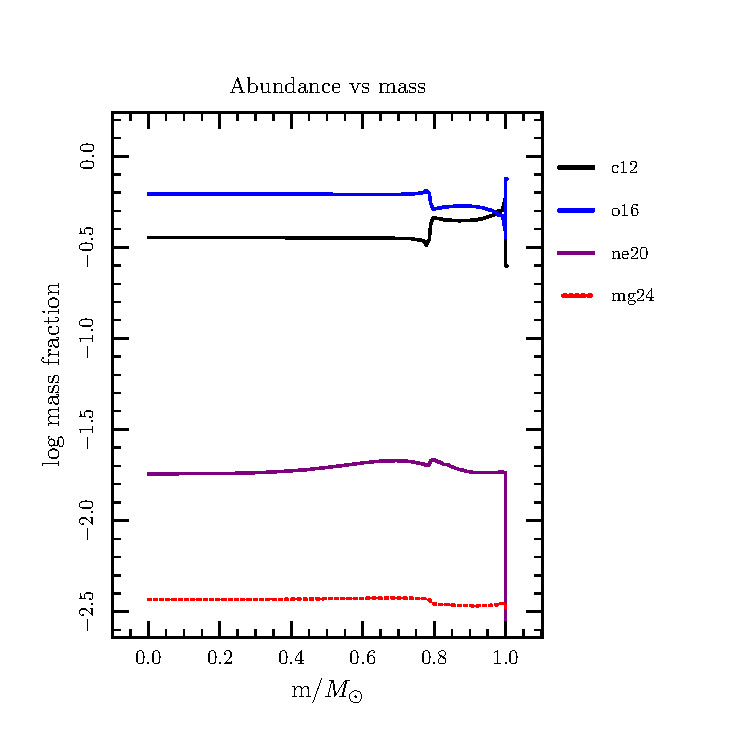
\includegraphics[width = 3.8in]{/Users/jaredbrooks/wd_ignite/plots_out/Abundance_vs_mass_1.pdf}
            \caption{Abundance profile shows mostly carbon and oxygen}
            \label{fig:2}
          \end{minipage}
	\end{figure}

        \pagebreak

        Because we are accreting carbon and oxygen and have negligible hydrogen and helium to begin with, there is no significant nuclear burning in the star until carbon and oxygen ignite at the end of the run.  Therefore, the smooth increases in luminosity and effective temperature, portrayed in the H.R. Diagram below(figure \ref{fig:3}), result from the release of gravitational potential energy from the accreting carbon and oxygen.  The temperature-density profile taken at a few ages (figure \ref{fig:7}) shows gradual increases in temperature and density until the core begins to heat rapidly.

        \begin{figure}[H]
          \begin{minipage}[b]{0.5\linewidth}
            \centering
            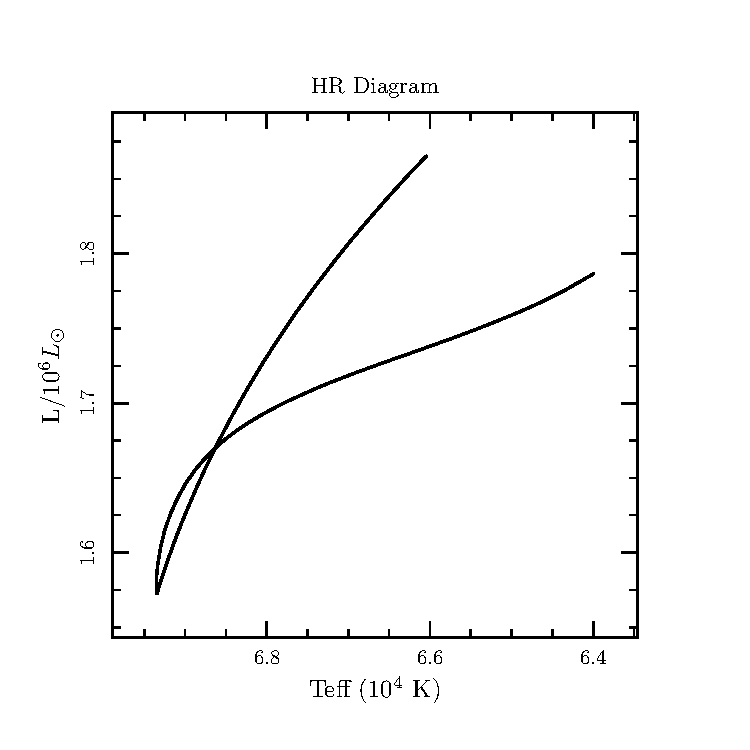
\includegraphics[width = 3.8in]{/Users/jaredbrooks/wd_ignite/plots_out/HR_Diagram.pdf}
            \caption{Smooth increases in luminosity and effective temperature due to release of gravitational potential energy from the accreting carbon and oxygen}
            \label{fig:3}
          \end{minipage}
          \hspace{0cm}
          \begin{minipage}[b]{0.5\linewidth}
            \centering
            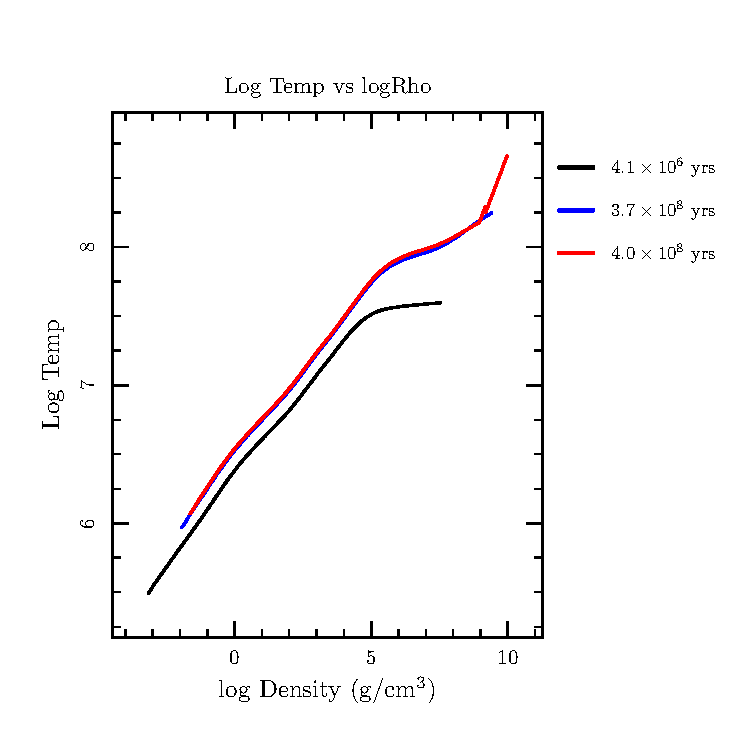
\includegraphics[width = 3.8in]{/Users/jaredbrooks/wd_ignite/plots_out/Log_Temp_vs_logRho.pdf}
            \caption{Temperature-density profile at a few ages}
            \label{fig:7}
          \end{minipage}
        \end{figure}
        
        \pagebreak

        This next profile (figure \ref{fig:4}) shows the burning rates right at the end of the run.  Only carbon and oxygen burning were high enough to show up on the plot, CNO and triple-alpha burning were too low.  The odd behavior at around m=0.8 can be explained by looking at the abundance plot at the end of the run.  There are two sharp composition boundaries near m=0.8, causing a disruption in the burning rates.

        \begin{figure}[H]
          \centering
          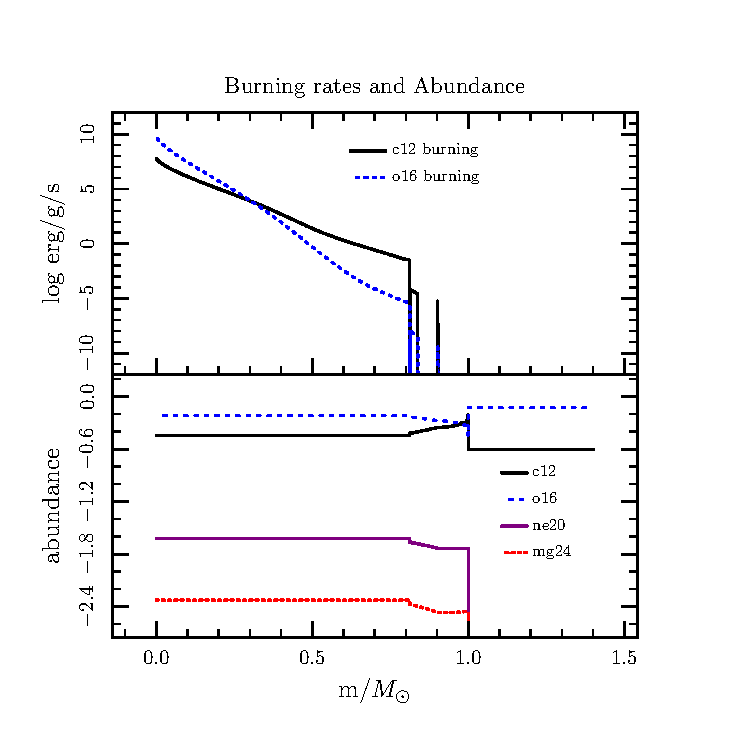
\includegraphics[width = 5in]{/Users/jaredbrooks/wd_ignite/plots_out/Burnrate_vs_mass.pdf}
          \caption{\footnotesize Carbon and oxygen burning strongest at the core, jumps near m=0.8}
          \label{fig:4}
        \end{figure}
        
        \pagebreak

        This final plot (figure \ref{fig:6}) shows a few internal \texttt{MESA} variables, such as the size of the time-step, the number of zones, and the number of retries against the model number in order to give some understanding of how hard \texttt{MESA} is working throughout the run and where some areas of problems/interest might be.

        \begin{figure}[H]
          \centering
          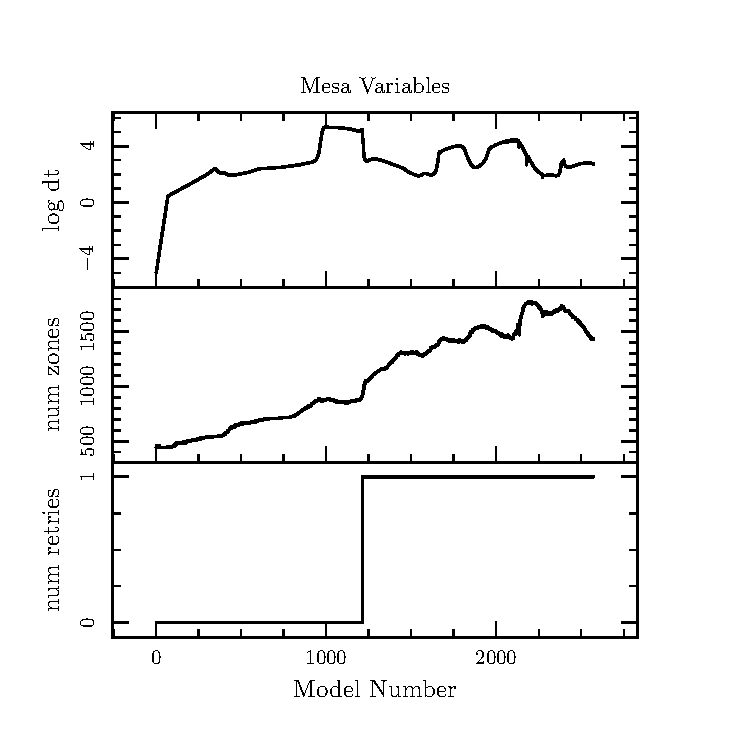
\includegraphics[width = 5in]{/Users/jaredbrooks/wd_ignite/plots_out/Mesa_Variables.pdf}
          \caption{\texttt{MESA} variables plotted against model number show how hard \texttt{MESA} is working}
          \label{fig:6}
        \end{figure}

\end{document}


